\section{Injective, Surjective, and Bijective}
We want to be able to describe the personalities of functions.  I encourage you to think of functions as if they have qualities, attributes, even personalities.  We want to have a vocabulary that describes attributes of functions to understand how they behave.  To this end we will begin with some definitions that, on the surface, seem silly and useless.  However, it is me hope that by the time we get through Cantor's proof you will have a fully developed, real life context for how these attributes are used.  I want us to find \emph{meaning} in these attributes. To be honest, this is something that I never had as a student; I was simply told to learn these definitions and apply them to totally stupid contexts, with only the most feable attempt by the teacher to provide context.  This whole discussion meant nothing to me and it wasn't until much later in my career that I formed an appreciation for the implications and meanings of these ideas.  I hope I do not become my teachers, and you don't have to become the student I once was.

Let us begin the discussion with the ideas of \emph{injective}, \emph{surjective}, and \emph{bijective}.

\subsection*{Relations that are functions}
\begin{definition}[Function] A function is a relation between $X$ and $Y$ denoted $$f: X\mapsto Y$$ for which  $$ f(x) = y_1 \land f(x) = y_2 \Rightarrow y_1=y_2.$$
\end{definition}


\begin{example}[Function]
Create an example of a relation from set $X$ to set $Y$ that is a function.  
%\notes{5}
\begin{figure}[ht]
\centering
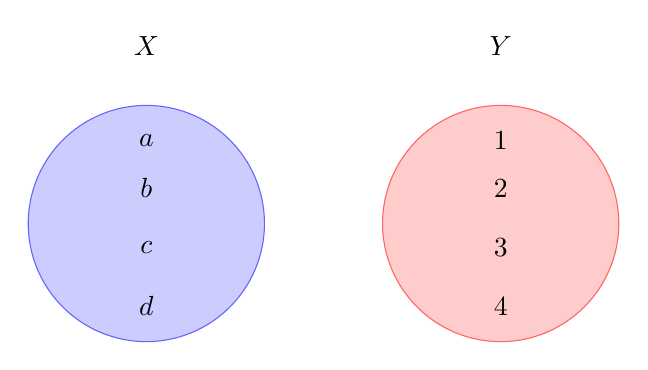
\begin{tikzpicture}[scale=1.50]
    % draw the sets
    \filldraw[fill=blue!20, draw=blue!60] (-1.5,0) circle (1cm);
    \filldraw[fill=red!20, draw=red!60] (1.5,0) circle (1cm);
    % the texts
    \node at (-1.5,1.5) {$X$};
    \node at (1.5,1.5) {$Y$};
    % the points in the sets (here I just create nodes to use them later on to position
    % the circles and the arrows
    \node (x1) at (-1.5,0.7) {$a$};
    \node (x2) at (-1.5,0.3) {$b$};
    \node (x3) at (-1.5,-0.2) {$c$};
    \node (x4) at (-1.5,-0.7) {$d$};
    \node (y1) at (1.5,0.7) {$1$};
    \node (y2) at (1.5,0.3) {$2$};
    \node (y3) at (1.5,-0.2) {$3$};
    \node (y4) at (1.5,-0.7) {$4$};
%    % draw the arrows
%    \draw[->] (x1) -- (y4);
%    \draw[->] (x2) -- (y2);
%    \draw[->] (x3) -- (y1);
%    \draw[->] (x4) -- (y3);
\end{tikzpicture}
%\caption{Mapping diagram of a relation that is a function.}
\end{figure}
Create a relation on $\mathbb{R}$ with this same property.
\begin{center}
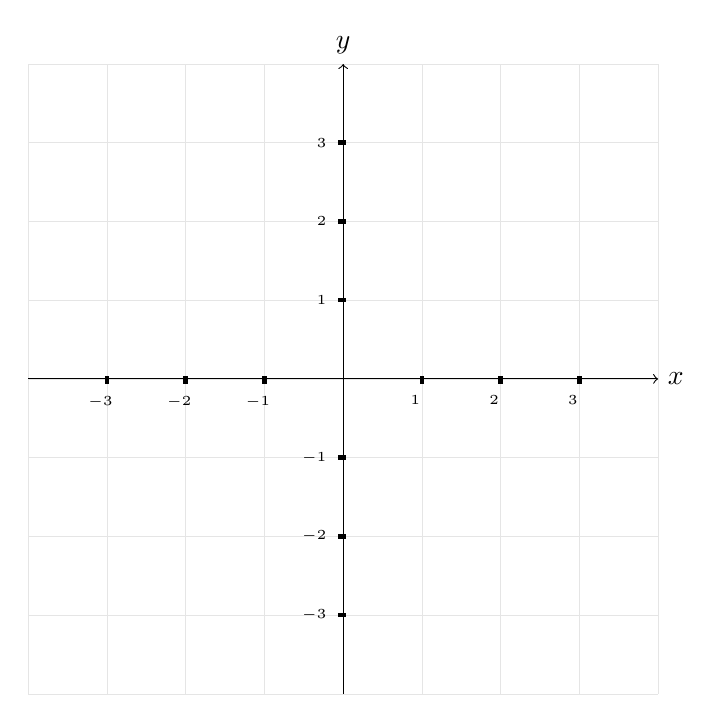
\begin{tikzpicture}[scale = 1.0]
\draw[ line width=0.2pt, black!10!white] (-4,-4) grid (4,4);
\draw[->] (-4,0) -- (4,0) node[right]{$x$};
\draw[->] (0,-4) -- (0,4) node[above]{$y$};
\foreach \x in {-3, -2,-1 ,1,2,3}
\draw[ultra thick] (\x*72/72,1pt) -- (\x*72/72,-2pt) node[anchor=north] {\tiny $ {\x}\ \ $};
\foreach \y in {-3, -2,-1 ,1,2,3}
	\draw[ultra thick] (1pt,\y) -- (-2pt,\y)
	node[anchor=east] {\tiny $\ \y$};
\end{tikzpicture}
\end{center}
\end{example}

\newpage
\begin{problem}[Not a function]
Create an example of a function from set $X$ to set $Y$ that is NOT a function.  
%\notes{5}
\begin{figure}[ht]
\centering
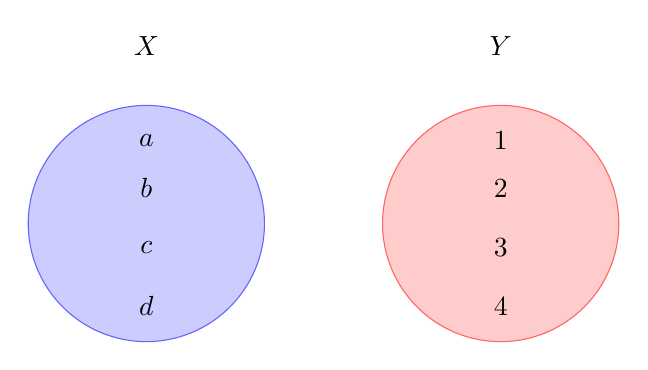
\begin{tikzpicture}[scale=1.50]
    % draw the sets
    \filldraw[fill=blue!20, draw=blue!60] (-1.5,0) circle (1cm);
    \filldraw[fill=red!20, draw=red!60] (1.5,0) circle (1cm);
    % the texts
    \node at (-1.5,1.5) {$X$};
    \node at (1.5,1.5) {$Y$};
    % the points in the sets (here I just create nodes to use them later on to position
    % the circles and the arrows
    \node (x1) at (-1.5,0.7) {$a$};
    \node (x2) at (-1.5,0.3) {$b$};
    \node (x3) at (-1.5,-0.2) {$c$};
    \node (x4) at (-1.5,-0.7) {$d$};
    \node (y1) at (1.5,0.7) {$1$};
    \node (y2) at (1.5,0.3) {$2$};
    \node (y3) at (1.5,-0.2) {$3$};
    \node (y4) at (1.5,-0.7) {$4$};
%    % draw the arrows
%    \draw[->] (x1) -- (y4);
%    \draw[->] (x2) -- (y2);
%    \draw[->] (x3) -- (y1);
%    \draw[->] (x4) -- (y3);
\end{tikzpicture}
%\caption{Mapping diagram of a relation that is not a function}
\end{figure}

Create a relation on $\mathbb{R}$ with this same property.
\begin{center}
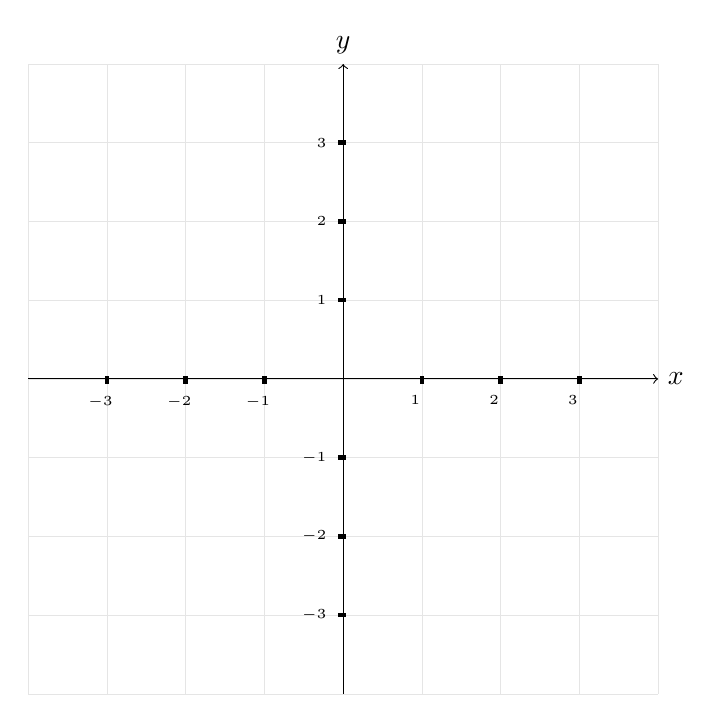
\begin{tikzpicture}[scale = 1.0]
\draw[ line width=0.2pt, black!10!white] (-4,-4) grid (4,4);
\draw[->] (-4,0) -- (4,0) node[right]{$x$};
\draw[->] (0,-4) -- (0,4) node[above]{$y$};
\foreach \x in {-3, -2,-1 ,1,2,3}
\draw[ultra thick] (\x*72/72,1pt) -- (\x*72/72,-2pt) node[anchor=north] {\tiny $ {\x}\ \ $};
\foreach \y in {-3, -2,-1 ,1,2,3}
	\draw[ultra thick] (1pt,\y) -- (-2pt,\y)
	node[anchor=east] {\tiny $\ \y$};
\end{tikzpicture}
\end{center}
\notes{10}
\end{problem}


\newpage

\subsection*{Injective}
\begin{definition}[Injective]
$$f(x) = f(y) \Rightarrow x = y.$$
\end{definition}
\begin{remark}  It might be worth noting that this is logically equivalent to the contrapositive, 
$$x \neq y \Rightarrow f(x) \neq f(y).$$
\end{remark}
\begin{example}[Injective]
Create an example of a function from set $X$ to set $Y$ that is injective.  
%\notes{5}
\begin{figure}[ht]
\centering
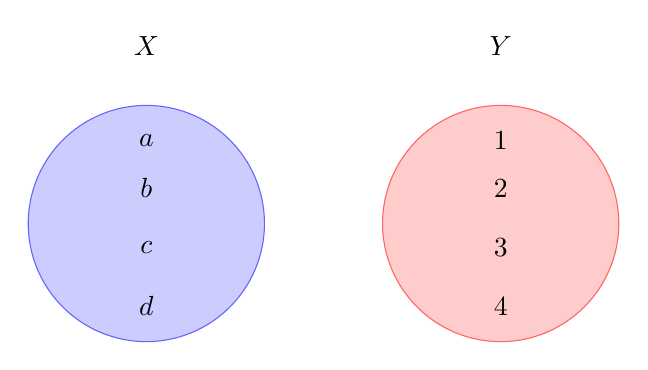
\begin{tikzpicture}[scale=1.50]
    % draw the sets
    \filldraw[fill=blue!20, draw=blue!60] (-1.5,0) circle (1cm);
    \filldraw[fill=red!20, draw=red!60] (1.5,0) circle (1cm);
    % the texts
    \node at (-1.5,1.5) {$X$};
    \node at (1.5,1.5) {$Y$};
    % the points in the sets (here I just create nodes to use them later on to position
    % the circles and the arrows
    \node (x1) at (-1.5,0.7) {$a$};
    \node (x2) at (-1.5,0.3) {$b$};
    \node (x3) at (-1.5,-0.2) {$c$};
    \node (x4) at (-1.5,-0.7) {$d$};
    \node (y1) at (1.5,0.7) {$1$};
    \node (y2) at (1.5,0.3) {$2$};
    \node (y3) at (1.5,-0.2) {$3$};
    \node (y4) at (1.5,-0.7) {$4$};
%    % draw the arrows
%    \draw[->] (x1) -- (y4);
%    \draw[->] (x2) -- (y2);
%    \draw[->] (x3) -- (y1);
%    \draw[->] (x4) -- (y3);
\end{tikzpicture}
%\caption{Mapping diagram of a relation that is injective}
\end{figure}

Create a relation on $\mathbb{R}$ with this same property.
\begin{center}
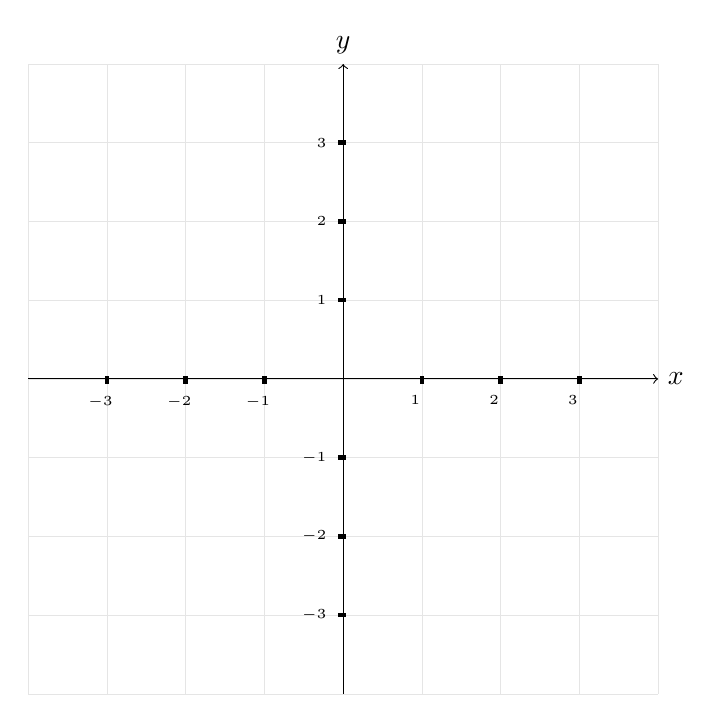
\begin{tikzpicture}[scale = 1.0]
\draw[ line width=0.2pt, black!10!white] (-4,-4) grid (4,4);
\draw[->] (-4,0) -- (4,0) node[right]{$x$};
\draw[->] (0,-4) -- (0,4) node[above]{$y$};
\foreach \x in {-3, -2,-1 ,1,2,3}
\draw[ultra thick] (\x*72/72,1pt) -- (\x*72/72,-2pt) node[anchor=north] {\tiny $ {\x}\ \ $};
\foreach \y in {-3, -2,-1 ,1,2,3}
	\draw[ultra thick] (1pt,\y) -- (-2pt,\y)
	node[anchor=east] {\tiny $\ \y$};
\end{tikzpicture}
\end{center}
\notes{5}
\end{example}

\newpage
\begin{problem}[Not Injective]
Create an example of a function from set $X$ to set $Y$ that is NOT injective.  
%\notes{5}
\begin{figure}[ht]
\centering
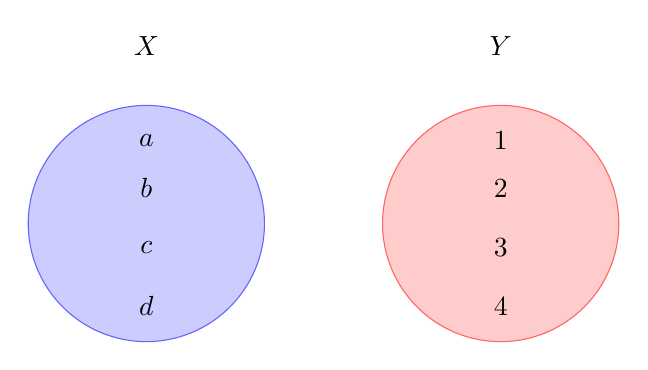
\begin{tikzpicture}[scale=1.50]
    % draw the sets
    \filldraw[fill=blue!20, draw=blue!60] (-1.5,0) circle (1cm);
    \filldraw[fill=red!20, draw=red!60] (1.5,0) circle (1cm);
    % the texts
    \node at (-1.5,1.5) {$X$};
    \node at (1.5,1.5) {$Y$};
    % the points in the sets (here I just create nodes to use them later on to position
    % the circles and the arrows
    \node (x1) at (-1.5,0.7) {$a$};
    \node (x2) at (-1.5,0.3) {$b$};
    \node (x3) at (-1.5,-0.2) {$c$};
    \node (x4) at (-1.5,-0.7) {$d$};
    \node (y1) at (1.5,0.7) {$1$};
    \node (y2) at (1.5,0.3) {$2$};
    \node (y3) at (1.5,-0.2) {$3$};
    \node (y4) at (1.5,-0.7) {$4$};
%    % draw the arrows
%    \draw[->] (x1) -- (y4);
%    \draw[->] (x2) -- (y2);
%    \draw[->] (x3) -- (y1);
%    \draw[->] (x4) -- (y3);
\end{tikzpicture}
%\caption{Mapping diagram of a relation that is not injective}
\end{figure}

Create a relation on $\mathbb{R}$ with this same property.
\begin{center}
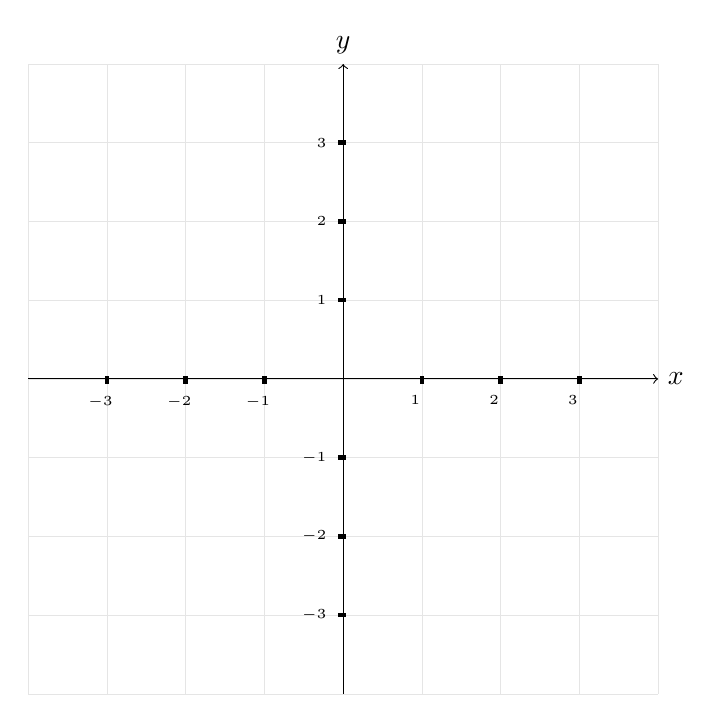
\begin{tikzpicture}[scale = 1.0]
\draw[ line width=0.2pt, black!10!white] (-4,-4) grid (4,4);
\draw[->] (-4,0) -- (4,0) node[right]{$x$};
\draw[->] (0,-4) -- (0,4) node[above]{$y$};
\foreach \x in {-3, -2,-1 ,1,2,3}
\draw[ultra thick] (\x*72/72,1pt) -- (\x*72/72,-2pt) node[anchor=north] {\tiny $ {\x}\ \ $};
\foreach \y in {-3, -2,-1 ,1,2,3}
	\draw[ultra thick] (1pt,\y) -- (-2pt,\y)
	node[anchor=east] {\tiny $\ \y$};
\end{tikzpicture}
\end{center}
\notes{10}
\end{problem}

\newpage
\subsection*{Surjective}
\begin{definition}[Surjective]
$$\forall ~y\in Y, ~\exists~x\in X \textrm{ such that } f(x) = y$$
\end{definition}

\begin{example}[Surjective]
Create an example of a function from set $X$ to set $Y$ that is surjective.  
%\notes{5}
\begin{figure}[ht]
\centering
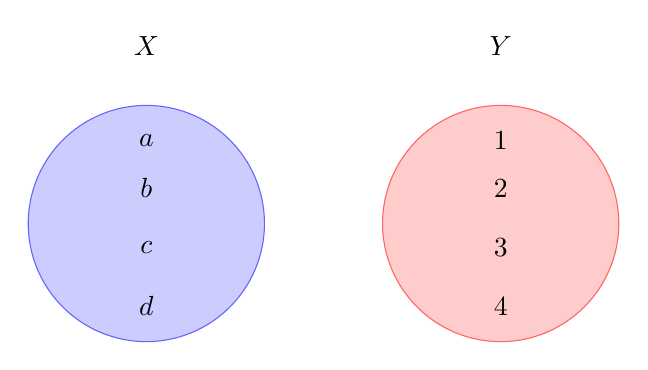
\begin{tikzpicture}[scale=1.50]
    % draw the sets
    \filldraw[fill=blue!20, draw=blue!60] (-1.5,0) circle (1cm);
    \filldraw[fill=red!20, draw=red!60] (1.5,0) circle (1cm);
    % the texts
    \node at (-1.5,1.5) {$X$};
    \node at (1.5,1.5) {$Y$};
    % the points in the sets (here I just create nodes to use them later on to position
    % the circles and the arrows
    \node (x1) at (-1.5,0.7) {$a$};
    \node (x2) at (-1.5,0.3) {$b$};
    \node (x3) at (-1.5,-0.2) {$c$};
    \node (x4) at (-1.5,-0.7) {$d$};
    \node (y1) at (1.5,0.7) {$1$};
    \node (y2) at (1.5,0.3) {$2$};
    \node (y3) at (1.5,-0.2) {$3$};
    \node (y4) at (1.5,-0.7) {$4$};
%    % draw the arrows
%    \draw[->] (x1) -- (y4);
%    \draw[->] (x2) -- (y2);
%    \draw[->] (x3) -- (y1);
%    \draw[->] (x4) -- (y3);
\end{tikzpicture}
%\caption{Mapping diagram of a relation that is surjective}
\end{figure}

Create a relation on $\mathbb{R}$ with this same property.
\begin{center}
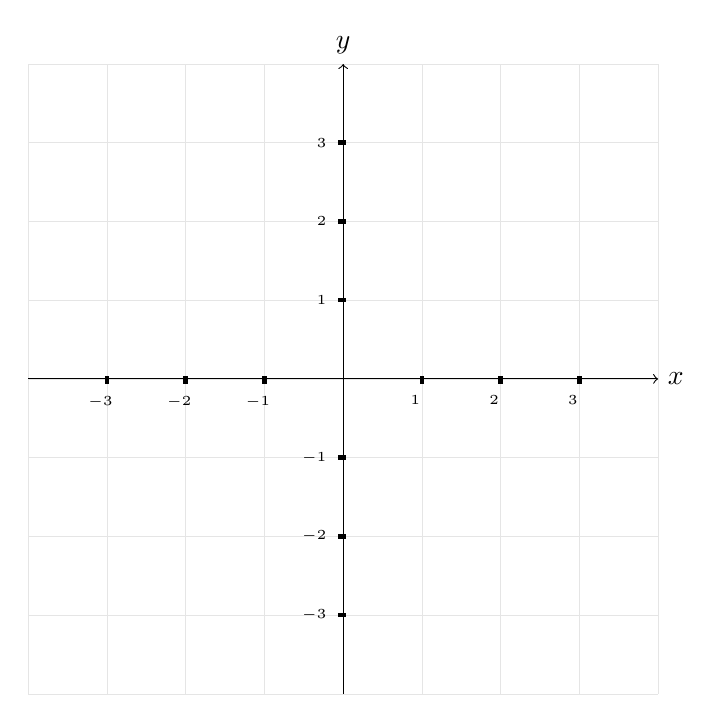
\begin{tikzpicture}[scale = 1.0]
\draw[ line width=0.2pt, black!10!white] (-4,-4) grid (4,4);
\draw[->] (-4,0) -- (4,0) node[right]{$x$};
\draw[->] (0,-4) -- (0,4) node[above]{$y$};
\foreach \x in {-3, -2,-1 ,1,2,3}
\draw[ultra thick] (\x*72/72,1pt) -- (\x*72/72,-2pt) node[anchor=north] {\tiny $ {\x}\ \ $};
\foreach \y in {-3, -2,-1 ,1,2,3}
	\draw[ultra thick] (1pt,\y) -- (-2pt,\y)
	node[anchor=east] {\tiny $\ \y$};
\end{tikzpicture}
\end{center}
\notes{10}
\end{example}

\newpage
\begin{problem}[Not surjective but is injective]
Create an example of a function from set $X$ to set $Y$ that is NOT surjective but is injective.  
%\notes{5}
\begin{figure}[ht]
\centering
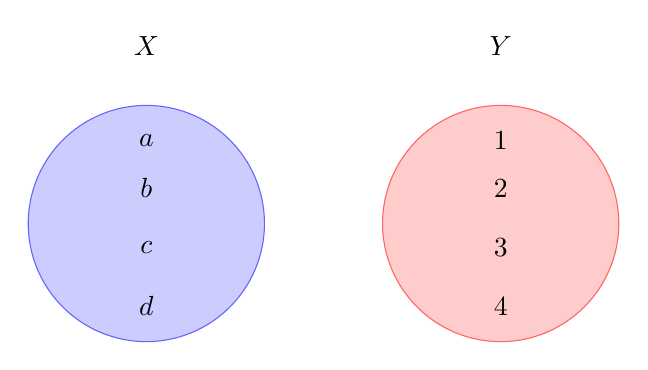
\begin{tikzpicture}[scale=1.50]
    % draw the sets
    \filldraw[fill=blue!20, draw=blue!60] (-1.5,0) circle (1cm);
    \filldraw[fill=red!20, draw=red!60] (1.5,0) circle (1cm);
    % the texts
    \node at (-1.5,1.5) {$X$};
    \node at (1.5,1.5) {$Y$};
    % the points in the sets (here I just create nodes to use them later on to position
    % the circles and the arrows
    \node (x1) at (-1.5,0.7) {$a$};
    \node (x2) at (-1.5,0.3) {$b$};
    \node (x3) at (-1.5,-0.2) {$c$};
    \node (x4) at (-1.5,-0.7) {$d$};
    \node (y1) at (1.5,0.7) {$1$};
    \node (y2) at (1.5,0.3) {$2$};
    \node (y3) at (1.5,-0.2) {$3$};
    \node (y4) at (1.5,-0.7) {$4$};
%    % draw the arrows
%    \draw[->] (x1) -- (y4);
%    \draw[->] (x2) -- (y2);
%    \draw[->] (x3) -- (y1);
%    \draw[->] (x4) -- (y3);
\end{tikzpicture}
%\caption{Mapping diagram of a relation that is surjective but not injective}
\end{figure}

Create a relation on $\mathbb{R}$ with this same property.
\begin{center}
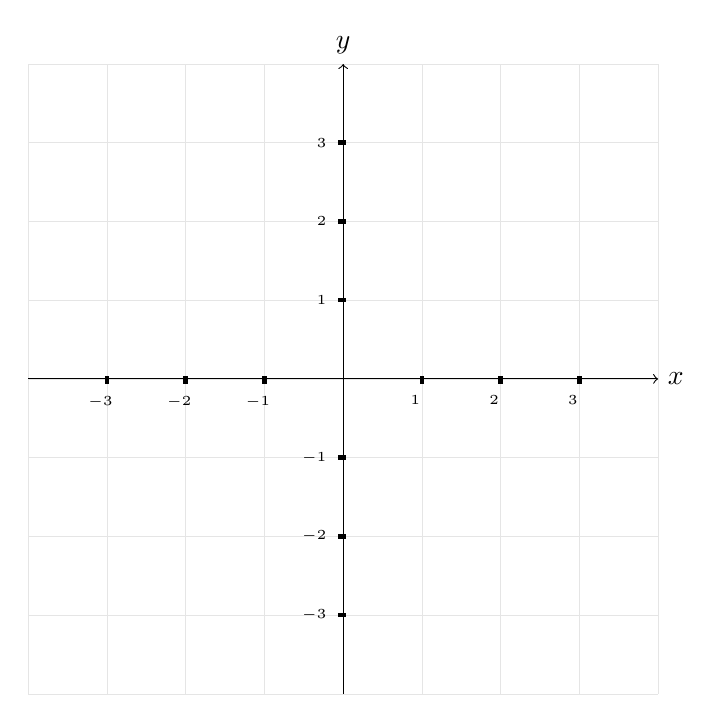
\begin{tikzpicture}[scale = 1.0]
\draw[ line width=0.2pt, black!10!white] (-4,-4) grid (4,4);
\draw[->] (-4,0) -- (4,0) node[right]{$x$};
\draw[->] (0,-4) -- (0,4) node[above]{$y$};
\foreach \x in {-3, -2,-1 ,1,2,3}
\draw[ultra thick] (\x*72/72,1pt) -- (\x*72/72,-2pt) node[anchor=north] {\tiny $ {\x}\ \ $};
\foreach \y in {-3, -2,-1 ,1,2,3}
	\draw[ultra thick] (1pt,\y) -- (-2pt,\y)
	node[anchor=east] {\tiny $\ \y$};
\end{tikzpicture}
\end{center}
\notes{10}
\end{problem}

\newpage
\begin{problem}[Surjective but not injective.]
Create an example of a function from set $X$ to set $Y$ that is surjective but NOT injective.  
%\notes{5}
\begin{figure}[ht]
\centering
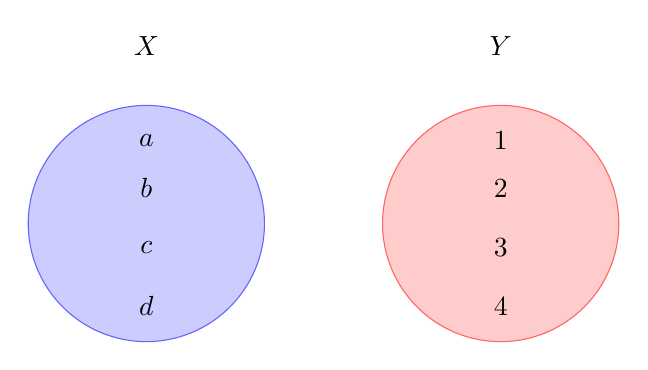
\begin{tikzpicture}[scale=1.50]
    % draw the sets
    \filldraw[fill=blue!20, draw=blue!60] (-1.5,0) circle (1cm);
    \filldraw[fill=red!20, draw=red!60] (1.5,0) circle (1cm);
    % the texts
    \node at (-1.5,1.5) {$X$};
    \node at (1.5,1.5) {$Y$};
    % the points in the sets (here I just create nodes to use them later on to position
    % the circles and the arrows
    \node (x1) at (-1.5,0.7) {$a$};
    \node (x2) at (-1.5,0.3) {$b$};
    \node (x3) at (-1.5,-0.2) {$c$};
    \node (x4) at (-1.5,-0.7) {$d$};
    \node (y1) at (1.5,0.7) {$1$};
    \node (y2) at (1.5,0.3) {$2$};
    \node (y3) at (1.5,-0.2) {$3$};
    \node (y4) at (1.5,-0.7) {$4$};
%    % draw the arrows
%    \draw[->] (x1) -- (y4);
%    \draw[->] (x2) -- (y2);
%    \draw[->] (x3) -- (y1);
%    \draw[->] (x4) -- (y3);
\end{tikzpicture}
%\caption{Mapping diagram of a relation that is surjective but not injective.}
\end{figure}

Create a relation on $\mathbb{R}$ with this same property.
\begin{center}
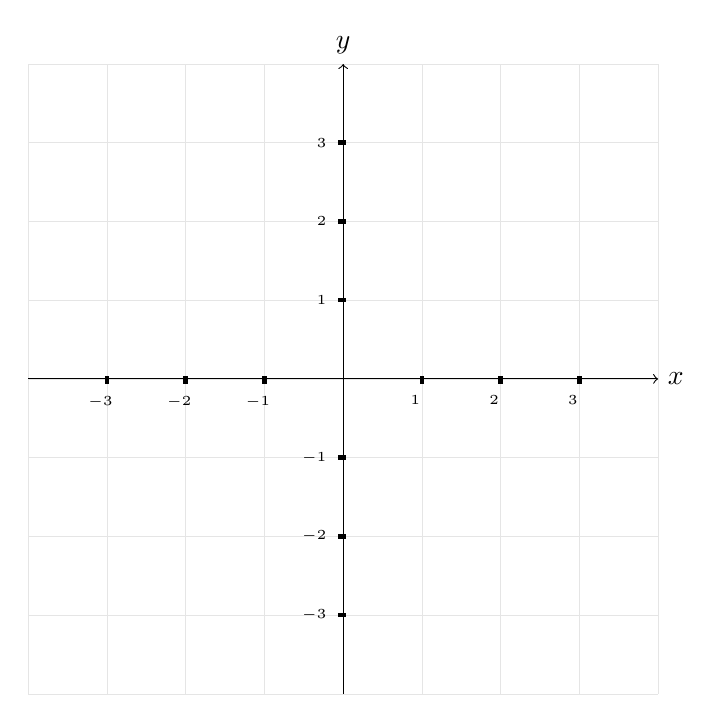
\begin{tikzpicture}[scale = 1.0]
\draw[ line width=0.2pt, black!10!white] (-4,-4) grid (4,4);
\draw[->] (-4,0) -- (4,0) node[right]{$x$};
\draw[->] (0,-4) -- (0,4) node[above]{$y$};
\foreach \x in {-3, -2,-1 ,1,2,3}
\draw[ultra thick] (\x*72/72,1pt) -- (\x*72/72,-2pt) node[anchor=north] {\tiny $ {\x}\ \ $};
\foreach \y in {-3, -2,-1 ,1,2,3}
	\draw[ultra thick] (1pt,\y) -- (-2pt,\y)
	node[anchor=east] {\tiny $\ \y$};
\end{tikzpicture}
\end{center}
\notes{10}
\end{problem}

\newpage
\subsection*{Bijective}
\begin{definition}[Bijective]
$$\forall ~y\in Y, ~\exists!~x\in X \textrm{ such that } f(x) = y$$

\end{definition}

\begin{example}[Bijective]
Create an example of a function from set $X$ to set $Y$ that is bijective.  
%\notes{5}
\begin{figure}[ht]
\centering
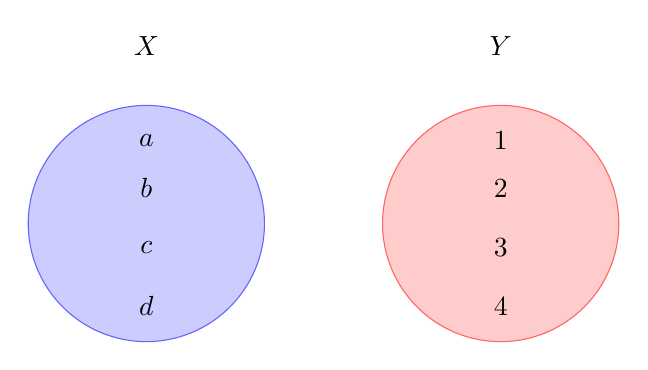
\begin{tikzpicture}[scale=1.50]
    % draw the sets
    \filldraw[fill=blue!20, draw=blue!60] (-1.5,0) circle (1cm);
    \filldraw[fill=red!20, draw=red!60] (1.5,0) circle (1cm);
    % the texts
    \node at (-1.5,1.5) {$X$};
    \node at (1.5,1.5) {$Y$};
    % the points in the sets (here I just create nodes to use them later on to position
    % the circles and the arrows
    \node (x1) at (-1.5,0.7) {$a$};
    \node (x2) at (-1.5,0.3) {$b$};
    \node (x3) at (-1.5,-0.2) {$c$};
    \node (x4) at (-1.5,-0.7) {$d$};
    \node (y1) at (1.5,0.7) {$1$};
    \node (y2) at (1.5,0.3) {$2$};
    \node (y3) at (1.5,-0.2) {$3$};
    \node (y4) at (1.5,-0.7) {$4$};
%    % draw the arrows
%    \draw[->] (x1) -- (y4);
%    \draw[->] (x2) -- (y2);
%    \draw[->] (x3) -- (y1);
%    \draw[->] (x4) -- (y3);
\end{tikzpicture}
%\caption{Mapping diagram of a relation that is bijective}
\end{figure}

Create a relation on $\mathbb{R}$ with this same property.
\begin{center}
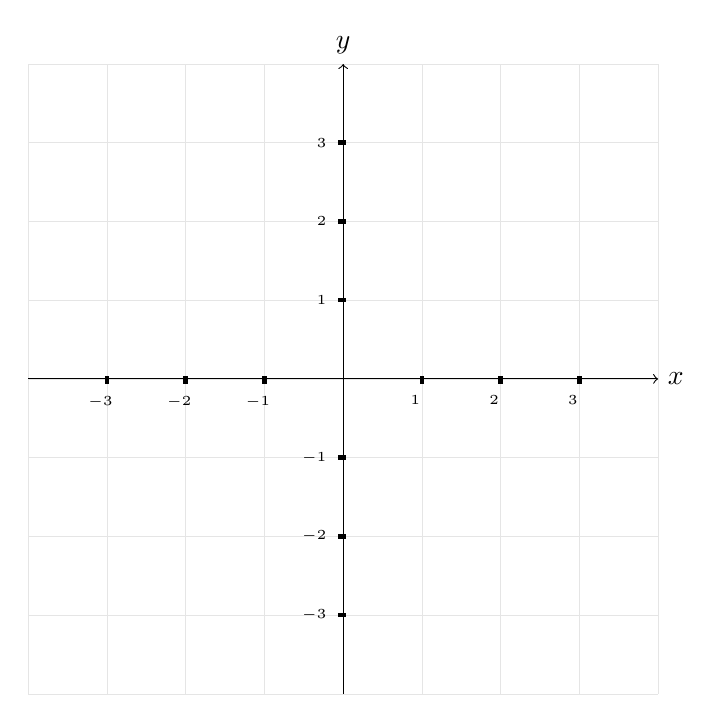
\begin{tikzpicture}[scale = 1.0]
\draw[ line width=0.2pt, black!10!white] (-4,-4) grid (4,4);
\draw[->] (-4,0) -- (4,0) node[right]{$x$};
\draw[->] (0,-4) -- (0,4) node[above]{$y$};
\foreach \x in {-3, -2,-1 ,1,2,3}
\draw[ultra thick] (\x*72/72,1pt) -- (\x*72/72,-2pt) node[anchor=north] {\tiny $ {\x}\ \ $};
\foreach \y in {-3, -2,-1 ,1,2,3}
	\draw[ultra thick] (1pt,\y) -- (-2pt,\y)
	node[anchor=east] {\tiny $\ \y$};
\end{tikzpicture}
\end{center}
\notes{10}
\end{example}

\newpage
\begin{problem}[Not bijective]
Create an example of a function from set $X$ to set $Y$ that is NOT bijective.  
%\notes{5}
\begin{figure}[ht]
\centering
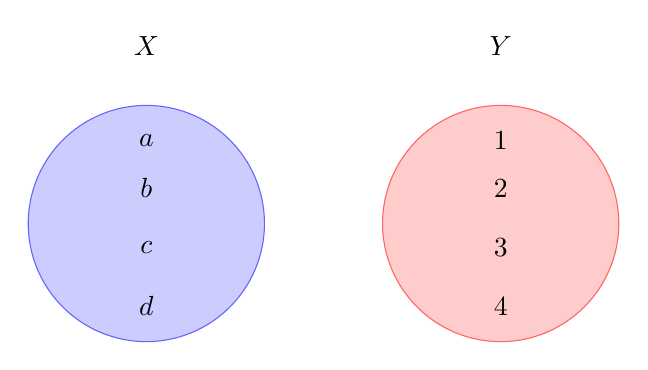
\begin{tikzpicture}[scale=1.50]
    % draw the sets
    \filldraw[fill=blue!20, draw=blue!60] (-1.5,0) circle (1cm);
    \filldraw[fill=red!20, draw=red!60] (1.5,0) circle (1cm);
    % the texts
    \node at (-1.5,1.5) {$X$};
    \node at (1.5,1.5) {$Y$};
    % the points in the sets (here I just create nodes to use them later on to position
    % the circles and the arrows
    \node (x1) at (-1.5,0.7) {$a$};
    \node (x2) at (-1.5,0.3) {$b$};
    \node (x3) at (-1.5,-0.2) {$c$};
    \node (x4) at (-1.5,-0.7) {$d$};
    \node (y1) at (1.5,0.7) {$1$};
    \node (y2) at (1.5,0.3) {$2$};
    \node (y3) at (1.5,-0.2) {$3$};
    \node (y4) at (1.5,-0.7) {$4$};
%    % draw the arrows
%    \draw[->] (x1) -- (y4);
%    \draw[->] (x2) -- (y2);
%    \draw[->] (x3) -- (y1);
%    \draw[->] (x4) -- (y3);
\end{tikzpicture}
%\caption{Mapping diagram of a relation that is bijective}
\end{figure}

Create a relation on $\mathbb{R}$ with this same property.
\begin{center}
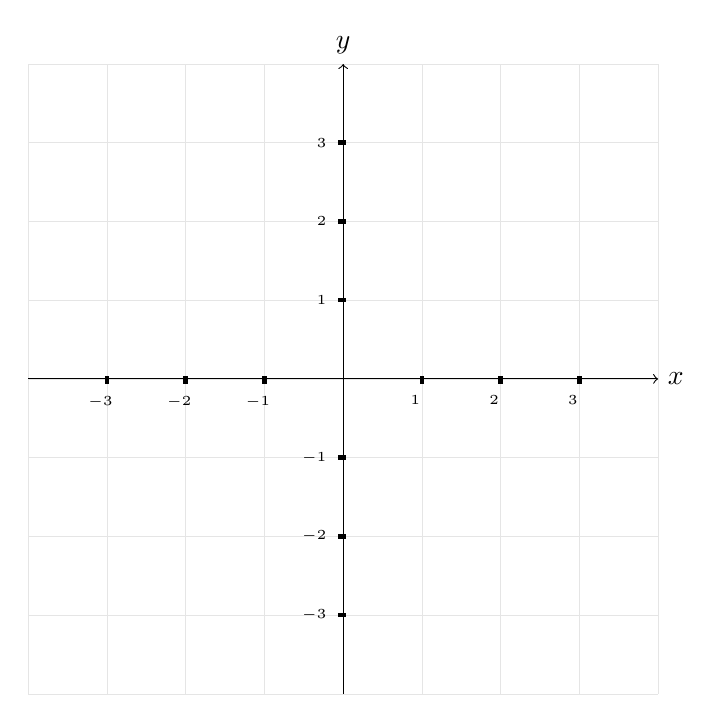
\begin{tikzpicture}[scale = 1.0]
\draw[ line width=0.2pt, black!10!white] (-4,-4) grid (4,4);
\draw[->] (-4,0) -- (4,0) node[right]{$x$};
\draw[->] (0,-4) -- (0,4) node[above]{$y$};
\foreach \x in {-3, -2,-1 ,1,2,3}
\draw[ultra thick] (\x*72/72,1pt) -- (\x*72/72,-2pt) node[anchor=north] {\tiny $ {\x}\ \ $};
\foreach \y in {-3, -2,-1 ,1,2,3}
	\draw[ultra thick] (1pt,\y) -- (-2pt,\y)
	node[anchor=east] {\tiny $\ \y$};
\end{tikzpicture}
\end{center}
\notes{10}
\end{problem}


